\chapter{Introduction to Model Comparison}\label{ch:model1}
%!TEX root = main.tex

A {\em model}\footnote{A similar term is {\em hypothesis}, and model comparison would then be {\em hypothesis testing}.  We don't choose to use that term, partly because of the colloquial use of hypothesis as a kind of ``guess,'' but also because hypothesis testing in some treatments focus on true/false tests of hypotheses which can lead to some significant misunderstandings.  The use of models implies the possibility of multiple (i.e. more than two) models.} as we use the term in this book is a {\em specific description of a possible state of nature}.  This is in contrast to an {\em actual} state of nature, which we practically never have access to.  We can never know {\em anything} with 100\% certainty, and must therefore be open to alternate possible explanations, or models, describing our observations.  For example, in medicine such models could include ``I have lung cancer,'' ``I have pneumonia,'' and ``I have a cold.''  In physics, models could include ``the Earth moves around the Sun'' and ``the Sun moves around the Earth.'' We can imagine many possible models that are consistent with the observed data, and our job in doing statistical inference is to determine the probabilities of our models given the data we observe.  In our notation, what we are always looking for is
\beq
P({\rm model}|{\rm data})
\label{eq:model_given_data}
\eeq

We will explore model comparison through a series of examples.


\section{The High/Low Deck Game}\label{sec:highlowdeck}

In this example we use a simple card game as a platform for discussing model comparison in general.  We start with two atypical decks of cards called the High Deck and the Low Deck (Figures~\ref{fig:highdeck} on page~\pageref{fig:highdeck} and \ref{fig:lowdeck} on page~\pageref{fig:lowdeck} respectively).  The game goes as follows. 
\begin{quote}
You're handed one of the two decks, but you don't know which.  First, you draw the top card and note the value.  Second, you replace the card and {\em reshuffle the deck}\footnote{Although we could make a game without replacement, which may be simpler to implement, the version of the game with reshuffling will help with an example later.}.  You repeat this procedure of drawing, noting, and reshuffling for as many turns as you need.  The goal is to determine which of the the two decks (High or Low) you are in fact holding in your hand.
\end{quote}

\begin{figure*}
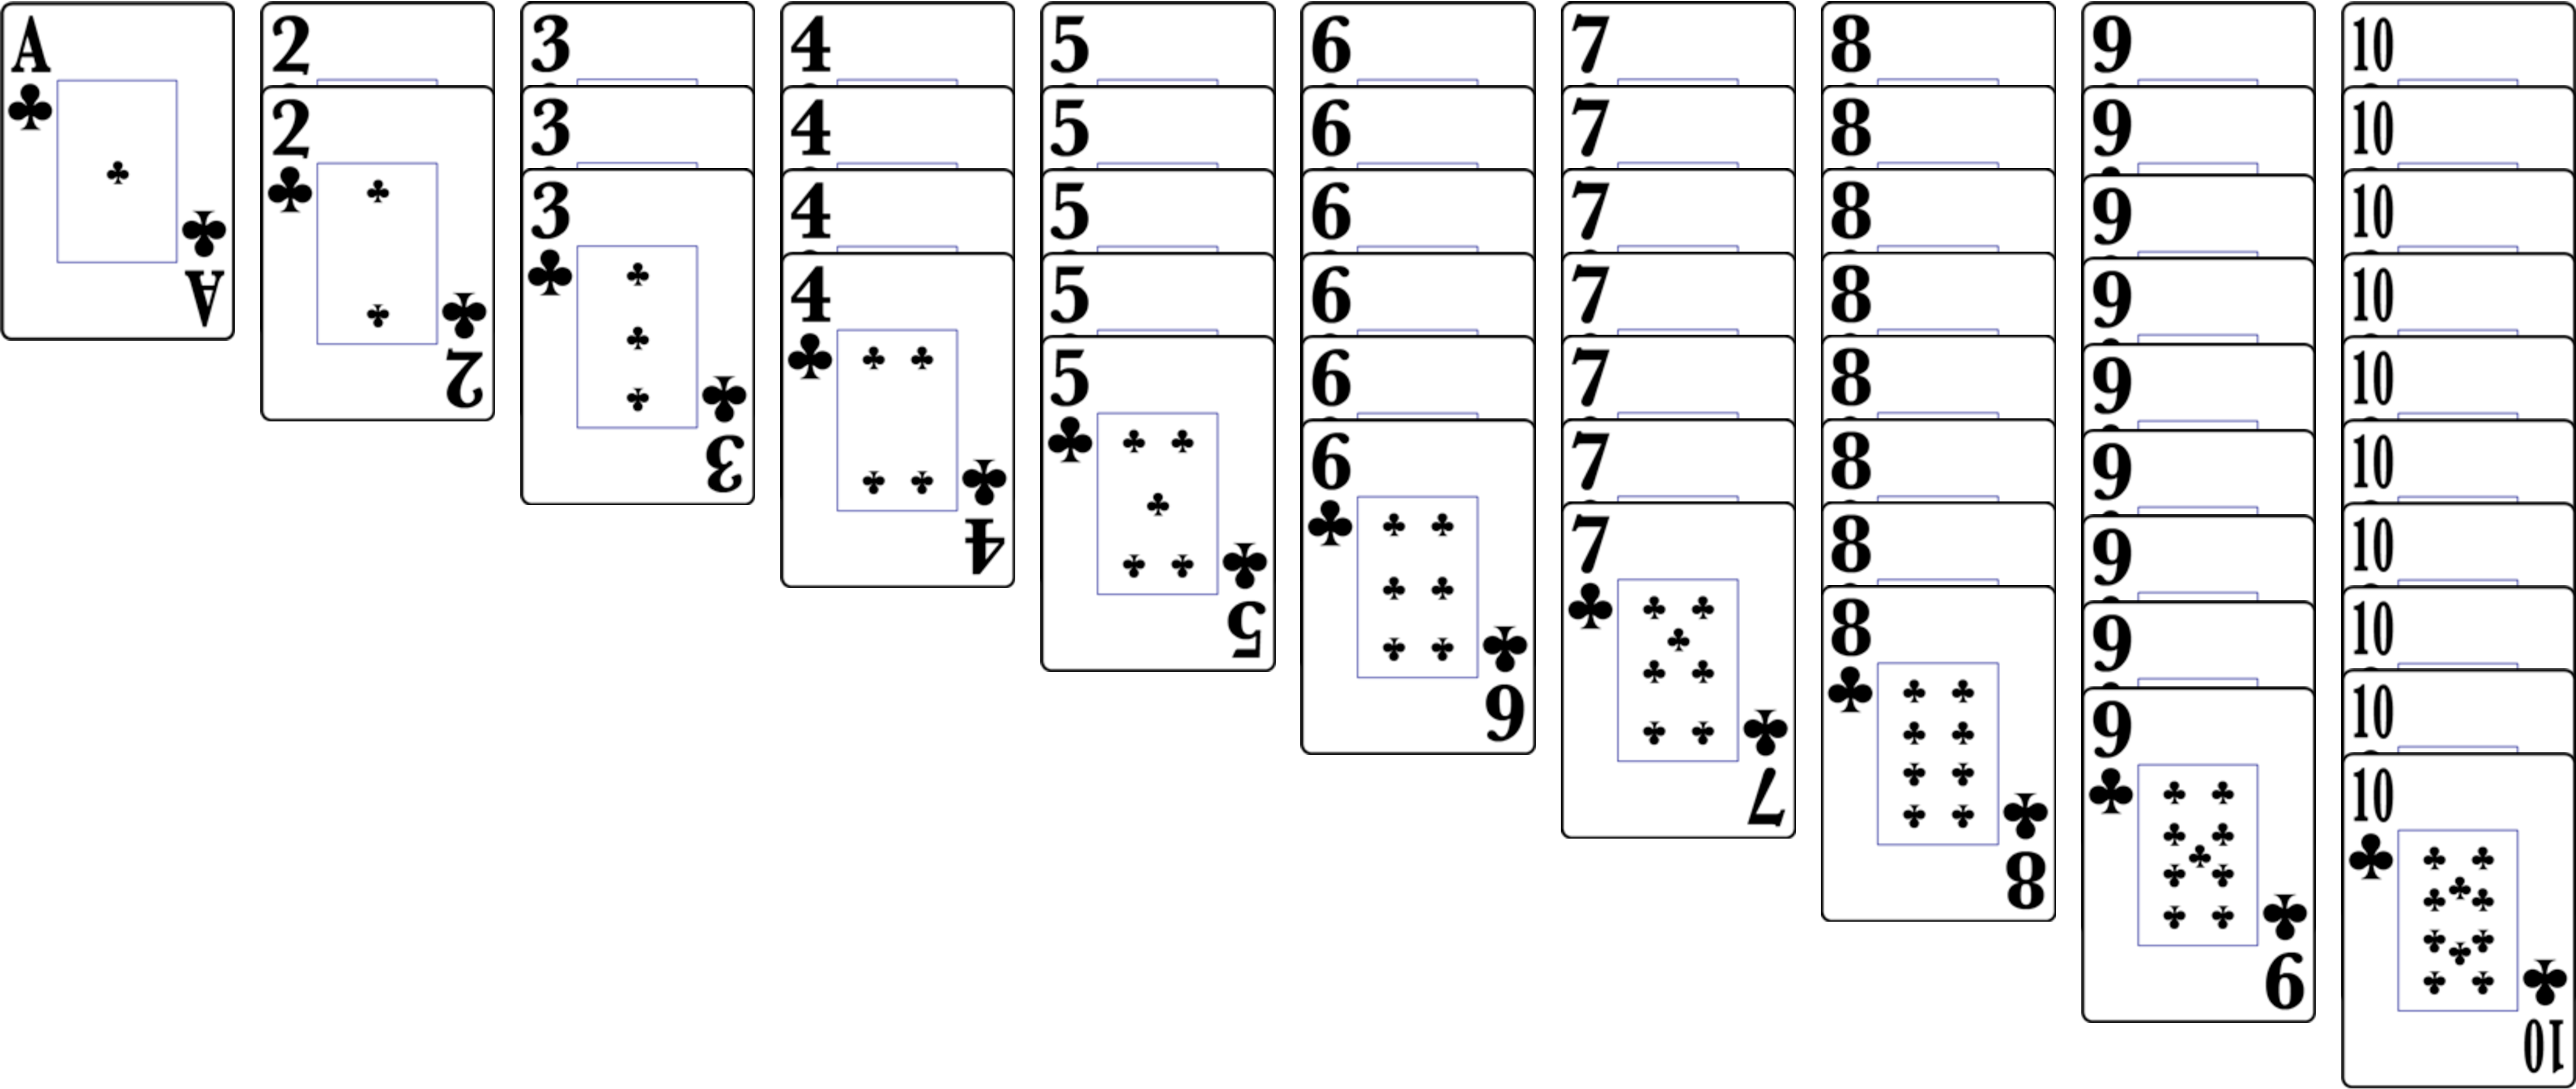
\includegraphics{HighDeck}
\caption{High Deck - 55 Cards with ten 10's, nine 9's, etc... down to one Ace.  Aces are equivalent to the value 1.}\label{fig:highdeck}
\end{figure*}

\begin{figure*}
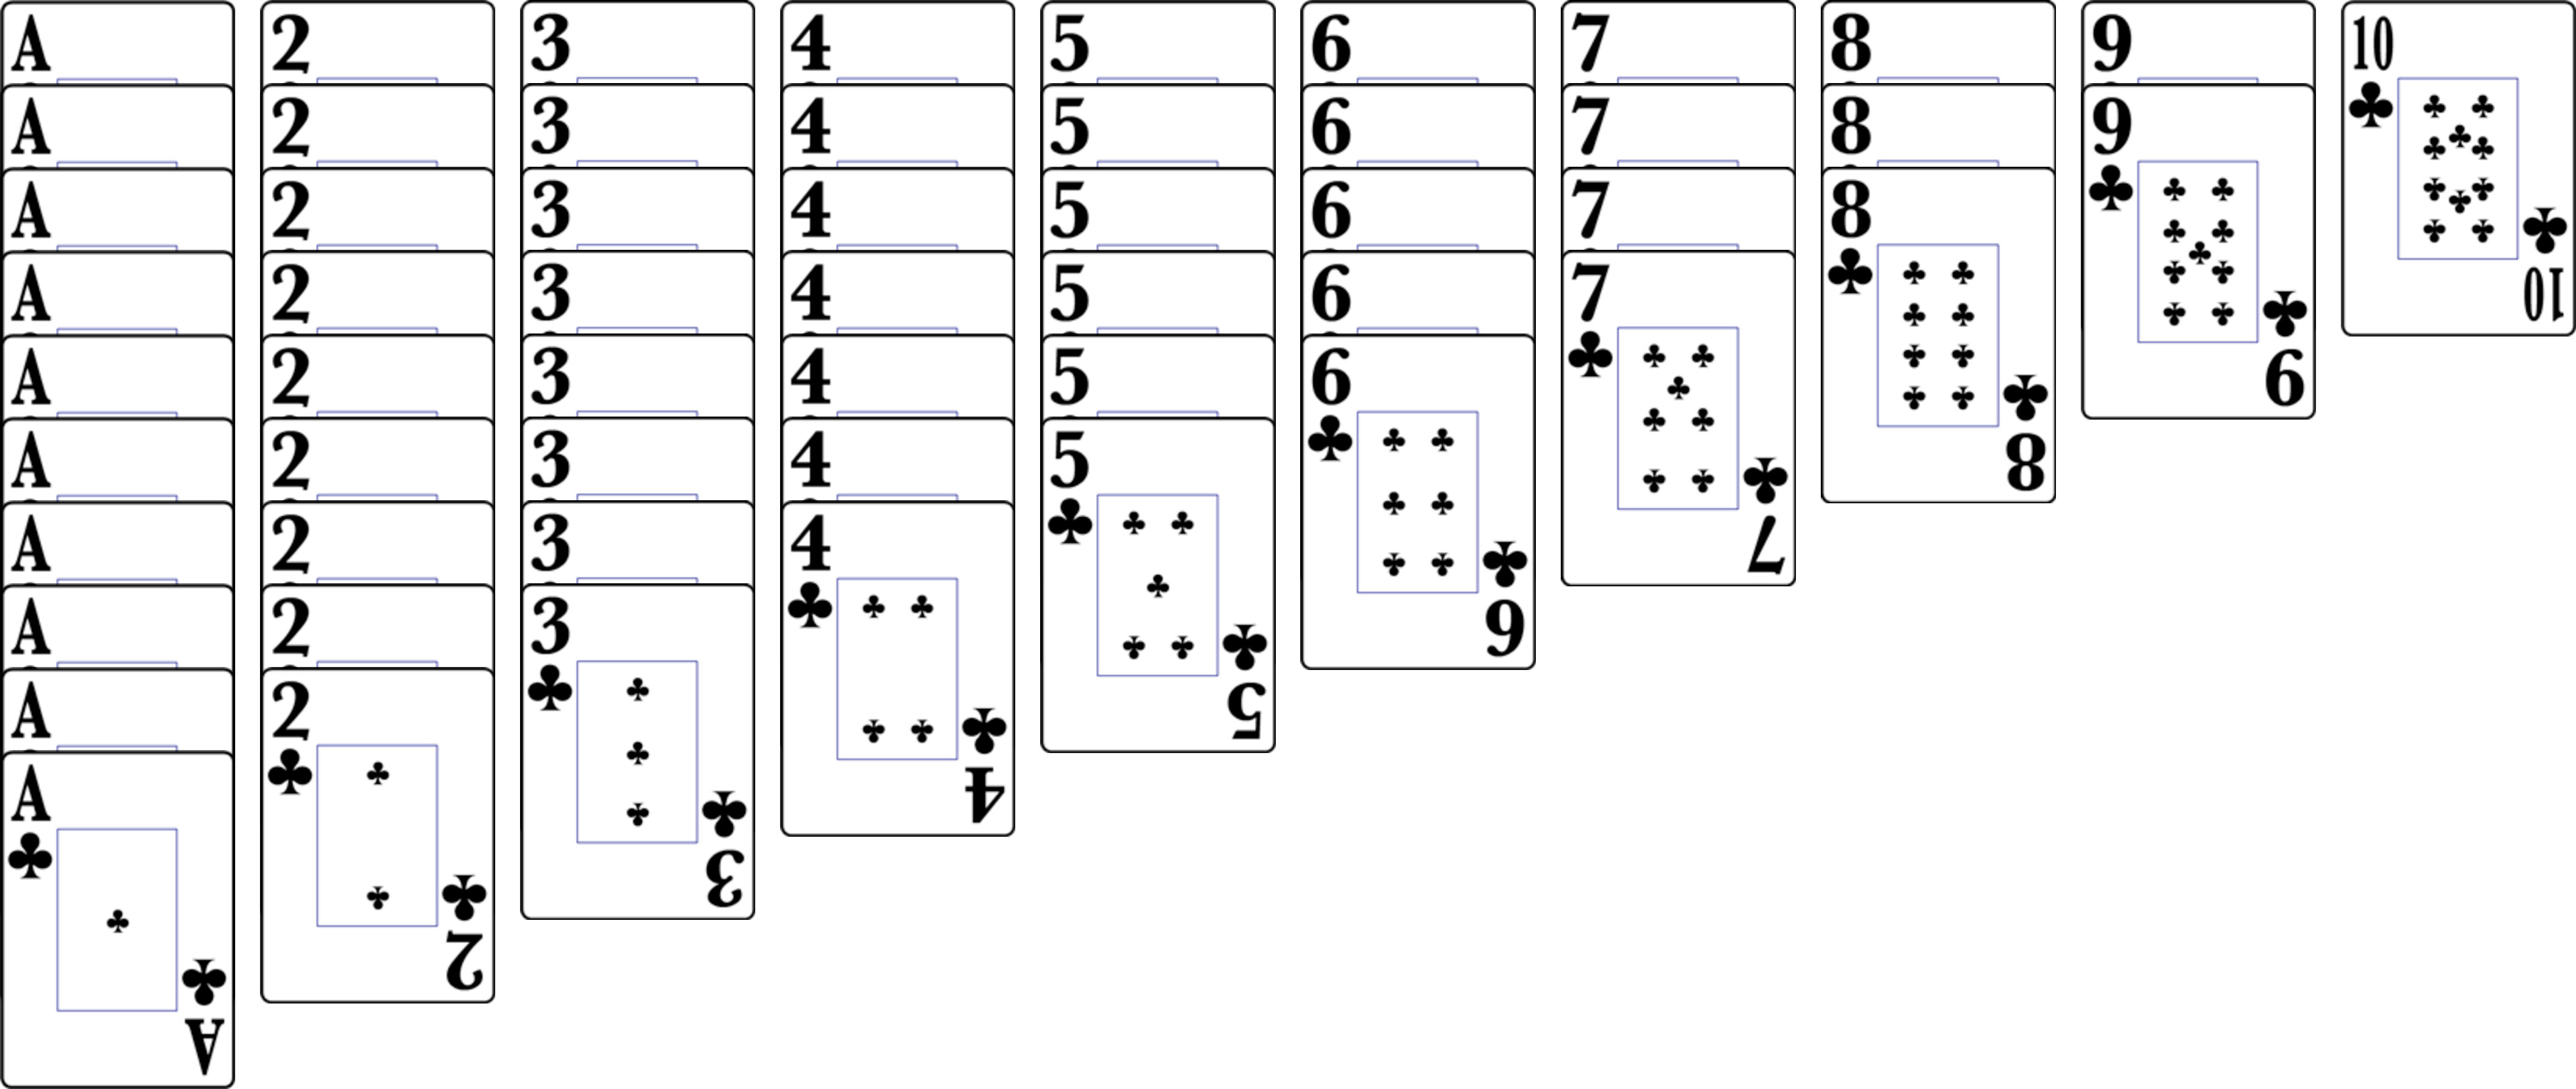
\includegraphics{LowDeck}
\caption{Low Deck - 55 Cards with ten Aces, two 2's, etc... up to one 10.  Aces are equivalent to the value 1.}\label{fig:lowdeck}
\end{figure*}



\subsection{What does our intuition say?}
We start by exploring our intuitions, before we do anything mathematically.  Thus, we are in a position to check to see if the math is reasonable before we use the same math in areas where our intuition is not as strong.  Imagine we draw only one card, and it is a 9.  Intuition suggests that this constitutes reasonably strong evidence toward the belief that we're holding the High Deck.  If we then (as the procedure states) place the 9 back in the deck, reshuffle and then draw a 7 we can be more strongly convinced that we are holding the High Deck.  Repeating the reshuffle, and then drawing a 3 would make us a little less confident in this conclusion, but still quite certain.  In this way we can sense how drawing different cards pushes our belief around, depending on how often that card comes up in the different decks.

\subsection{Before the data - the prior}

Before we take any data, we need to quantify our state of knowledge concerning all of the models that we are considering.  In this case it is quite simple, because there are two models (High Deck and Low Deck), and we have been given no information about whether either is more common.  With no such information, it is equivalent to a coin flip - we assign equal probabilities to both models {\em before} we see data, also known as the {\em prior} probabilities\footnote{The prior is sometimes mischaracterized as simply our guess, or some other completely subjective assessment of our knowledge.  In fact in this example, and many others, we can make the {\em positive} case for equal probabilities given the state of our knowledge.  This can be quantified with the concept of entropy, which is beyond this chapter.}.  
\beqn
P(H) &=& 0.5 \\
P(L) &=& 0.5
\eeqn
Surely this assessment will change {\em after} we see data, but that is the rest of the problem.

\subsection{The ``easy'' question - the likelihood}

Although our ultimate goal is to infer the type of deck from the cards that we draw from it, we can start looking at an easier part of this question which serves as a first step toward the more challenging, and interesting goal.  That question is the following, 
\example{What is the probability of drawing a 9, given that we know that we're holding the High Deck?
}
This related question is written
\beqn
P({\rm data}=9|H)
\eeqn
where ${\rm data}=9$ means that we have observed (i.e. drawn) one 9.  This question is ``easy'' in the sense that it is simply related to the properties of the High Deck: the number of 9's and total number of cards.  If you know that you have the high deck, then you know there are nine 9's in that deck out of 55 cards, and thus we have the probability of drawing one 9, given that we are holding the High Deck, is
\beqn
P({\rm data}=9|H)=\frac{9}{55}
\eeqn
We give this the name {\em likelihood}\footnote{The term {\em likelihood} is a poorly chosen word.  In English, this word is nearly synonymous with the word {\em probability} and thus easily leads to confusion.  We could try to use a different term, like {\em consequent probability} or {\em generative likelihood} to stress the idea that the {\em likelihood} is the probability that the data we observe could be generated or could be a consequence of the particular model.  However, we'd be going up against two centuries of continued use of the term {\em likelihood} and thus would probably increase confusion rather than decrease it.}, and is simply the probability that the data could be the result of a known model.  It is also the first part of the top of Bayes' Rule, Equation~\ref{eq:bayes} on page~\pageref{eq:bayes}.


\subsection{Applying the Bayes' recipe}

Here we introduce for the first time a recipe we will follow for all model comparison examples.

Now that we have our intuition, and we have the likelihoods, we can address the math.  The two models are:
\beqn
H&\equiv& \mbox{``We're holding the High Deck''}\\
L&\equiv& \mbox{``We're holding the Low Deck''}
\eeqn
and the initial data is
\beqn
{\rm data}&\equiv& \mbox{``We've drawn one card, and it is a 9''}\\
\eeqn
According to Equation~\ref{eq:model_given_data} on page~\pageref{eq:model_given_data} we are looking for the two probabilities:
\beqn
P(H|{\rm data}=\emph{9}) \\
P(L|{\rm data}=\emph{9}) 
\eeqn
which are related to the {\em prior} and the {\em likelihood} via Bayes' Rule (Equation~\ref{eq:bayes}):
\beqn
P(H|{\rm data}=9)&=&\frac{P({\rm data}=9|H)P(H)}{P({\rm data}=9)}\\
P(L|{\rm data}=9)&=&\frac{P({\rm data}=9|L)P(L)}{P({\rm data}=9)} 
\eeqn

To calculate actual numbers, we apply the Bayes' Recipe to this problem,
\be
\i Specify the prior probabilities for the models being considered
\beqn
P(H) &=& 0.5 \\
P(L) &=& 0.5
\eeqn
\i Write the top of Bayes' Rule for all models being considered
\beqn
P(H|{\rm data}=9)&\sim& P({\rm data}=9|H)P(H) \\
P(L|{\rm data}=9)&\sim& P({\rm data}=9|L)P(L) 
\eeqn
where we are using the symbol $\sim$ to denote {\em proportionality} or {\em related to}.  Essentially, by calculating the top of Bayes' Rule first, the numbers are not {\em equal} to the final (i.e. posterior) probabilities but must be rescaled to make sure that they add up to 1.  This is done in the final step.  Up until that rescaling, we use the symbol $\sim$ and think of it as {\em related to}.
\i Put in the likelihood and prior values
\beqn
P(H|{\rm data}=9)&\sim& \frac{9}{55}\times 0.5 =0.082 \\
P(L|{\rm data}=9)&\sim& \frac{2}{55}\times 0.5 =0.018 
\eeqn
\i Add these values for all models
\beqn
K=0.082+0.018 = 0.1
\eeqn
\i Divide each of the values by this sum, $K$, to get the final probabilities
\beqn
P(H|{\rm data})=0.082/0.1 = 0.82\\
P(L|{\rm data})=0.018 /0.1 = 0.18
\eeqn
\ee

From which we can conclude that drawing a 9 does indeed constitute reasonably strong evidence toward the belief that we're holding the High Deck - the probability of us holding the High Deck, given the data, is 0.82.

\subsection{Drawing the next card}

So, when we draw a 7 next (after reshuffling), our intuition suggests that we'd be more confident that we're holding the High Deck.  Repeating our recipe we have

The two models are:
\beqn
H&\equiv& \mbox{``We're holding the High Deck''}\\
L&\equiv& \mbox{``We're holding the Low Deck''}
\eeqn
and data is
\beqn
{\rm data}&\equiv& \left\{\parbox{3in}{``We've drawn one card, and it is a 9, replaced and reshuffled, and then drawn a 7''}\right.\\
\eeqn
According to Equation~\ref{eq:model_given_data} we are looking for the two probabilities:
\beqn
P(H|{\rm data}=9\mbox{ then a }7) \\
P(L|{\rm data}=9\mbox{ then a 7}) 
\eeqn
which are related to the {\em prior} and the {\em likelihood} via Bayes' Rule (Equation~\ref{eq:bayes}):
\beqn
P(H|{\rm data}=9\mbox{ then a }7)&=&\frac{P({\rm data}=9\mbox{ then a }7|H)P(H)}{P({\rm data}=9\mbox{ then a }7)}\\
P(L|{\rm data}=9\mbox{ then a }7)&=&\frac{P({\rm data}=9\mbox{ then a }7|L)P(L)}{P({\rm data}=9\mbox{ then a }7)} 
\eeqn

To calculate actual numbers, we apply the Bayes' recipe to this problem,
\be
\i Specify the prior probabilities for the models being considered
\beqn
P(H) &=& 0.5 \\
P(L) &=& 0.5
\eeqn
\i Write the top of Bayes' Rule for all models being considered
\beqn
P(H|{\rm data}=9\mbox{ then a }7)&\sim& P({\rm data}=9\mbox{ then a }7|H)P(H) \\
P(L|{\rm data}=9\mbox{ then a }7)&\sim& P({\rm data}=9\mbox{ then a }7|L)P(L) 
\eeqn
\i Put in the likelihood and prior values\marginnote{As a reminder, we are performing this next draw {\em having shuffled the first draw back into the deck}.  Although somewhat artificial, it is useful for a later example.  If we had simply set the first card asside, the value of the likelihood would account for the removal of one more card, and would thus be $\frac{9}{55}\times\frac{7}{{\bf 54}}$ for the high deck and $\frac{2}{55}\times\frac{4}{{\bf 54}}$ for the low deck. Note the denominators.}
\beqn
P(H|{\rm data}=9\mbox{ then a }7)&\sim& \frac{9}{55}\times\frac{7}{55}\times 0.5 =0.0104 \\
P(L|{\rm data}=9\mbox{ then a }7)&\sim& \frac{2}{55}\times\frac{4}{55}\times 0.5 =0.0013 
\eeqn
\i Add these values for all models
\beqn
K=0.0104+0.0013 = 0.0117
\eeqn
\i Divide each of the values by this sum, $K$, to get the final probabilities
\beqn
P(H|{\rm data}=9\mbox{ then a }7)=0.0104/0.0117 =0.889 \\
P(L|{\rm data}=9\mbox{ then a }7)=0.0013/0.0117 =0.111 
\eeqn
\ee

which again matches our intuition - we're more confident that we're holding the High Deck, now with probability 0.889 increased from 0.82 when we just observed the 9. 

\subsection{Prior information or not?}

In the above example, we started with a prior probability of holding the High Deck at $P(H)=0.5$, because we had no information other than that there were two possibilities.  We then observed a 9, and updated the probability to 0.82, and then observed a 7, and further updated the probability to 0.889 - making it more likely that we were holding the High Deck.  One of the basic tenets of probability theory is that if there is more than one way to arrive at an answer, one should arrive at the same answer.\footnote{E. T. Jaynes uses the principle that ``if there is more than one way to arrive at an answer, one should arrive at the same answer'' to help derive the rules of probability from first principles.  Failures of this principle result in paradoxes.  This principle is also applied in Section~\ref{sec:birthday} for the birthday problem.}  In the above, we calculated the probability of holding the High Deck given the observed data
\beqn
{\rm data}&\equiv&\left\{ \parbox{3in}{``We've drawn one card, and it is a 9, replaced and reshuffled, and then drawn a 7''}\right.\\
\eeqn
and prior information
\beqn
{\rm prior}&\equiv& \parbox{3in}{``We know there are only two decks.''}\\
\eeqn

An equivalent situation is found after our first draw, after we've observed the 9, and we're about to draw our second card.  In this case we have the {\em prior} information:
\beqn
{\rm prior}&\equiv& \left\{\parbox{3in}{``We know there are only two decks, and then we draw one card and it is a 9, replace it and reshuffle.''}\right.\\
\eeqn
and observed data:
\beqn
{\rm data}&\equiv& \parbox{3in}{``We've drawn one card and it is a 7''}\\
\eeqn

Mathematically, we apply the Bayes' recipe, but with the different prior information
\be
\i Specify the prior probabilities for the models being considered
\beqn
P(H,9) &=& 0.82 \\
P(L,9) &=& 0.18
\eeqn
\i Write the top of Bayes' Rule for all models being considered
\beqn
P(H|{\rm data}=9\mbox{ then a }7)&\sim& P({\rm data}=7|H)P(H,9) \\
P(L|{\rm data}=9\mbox{ then a }7)&\sim& P({\rm data}=7|L)P(L,9) 
\eeqn
\i Put in the likelihood and prior values
\beqn
P(H|{\rm data}=9\mbox{ then a }7)&\sim& \frac{7}{55}\times 0.82 =0.104 \\
P(L|{\rm data}=9\mbox{ then a }7)&\sim& \frac{4}{55}\times 0.18 =0.013
\eeqn
\i Add these values for all models
\beqn
K=0.104+0.013 = 0.117
\eeqn
\i Divide each of the values by this sum, $K$, to get the final probabilities
\beqn
P(H|{\rm data}=9\mbox{ then a }7)=0.104/0.117 =0.889 \\
P(L|{\rm data}=9\mbox{ then a }7)=0.013/0.117 =0.111 
\eeqn
\ee
yielding the same result.

In other words our {\em updated probabilities} from the first draw can be seen as our {\rm prior} probabilities for the subsequent draws.  Thus, Bayes' Rule describes how we update our knowledge with new evidence, or in other words, \emph{learning}.

\section{Multiple Hypotheses}\label{sec:multiplehypotheses}

We start this section with an example.

\example{What is the probability that you are holding one of either the High or the Low Deck having drawn five 9's in a row from that deck?}

We have observed the following data:
\beqn
{\rm data}&\equiv& \left\{\parbox{3in}{``We've drawn one card, and it is a 9, replaced and reshuffled, redrawn and observed another 9, repeated this procedure and observed three more 9's, for a total of five 9's in a row.''}\right.
\eeqn
Technically, drawing 5 9's in a row should give us really strong confidence that you are drawing from the High Deck, because we would have
\be
\i Specify the prior probabilities for the models being considered
\beqn
P(H) &=& 0.5 \\
P(L) &=& 0.5
\eeqn
\i Write the top of Bayes' Rule for all models being considered
\beqn
P(H|{\rm data}=5\mbox{ 9's in a row})&\sim& P({\rm data}=5\mbox{ 9's in a row}|H)P(H) \\
P(L|{\rm data}=5\mbox{ 9's in a row})&\sim& P({\rm data}=5\mbox{ 9's in a row}|L)P(L) 
\eeqn
\i Put in the likelihood and prior values
\beqn
P(H|{\rm data}=5\mbox{ 9's in a row})&\sim&\underbrace{\frac{9}{55}\times\frac{9}{55}\cdots\frac{9}{55}}_{5\mbox{ times}} \times P(H)\\
&\sim& \left(\frac{9}{55}\right)^{5}\times 0.5 \\
&=&0.0000587\\
P(L|{\rm data}=5\mbox{ 9's in a row})&\sim& \left(\frac{2}{55}\right)^{5}\times 0.5\\
&=&0.0000000318
\eeqn
\i Add these values for all models
\beqn
K=0.0000587+0.0000000318 = 0.0000587318
\eeqn
\i Divide each of the values by this sum, $K$, to get the final probabilities
\beqn
P(H|{\rm data}=5\mbox{ 9's in a row})&=& \frac{0.0000587}{0.0000587318}=0.99946\\
P(L|{\rm data}=5\mbox{ 9's in a row})&=& \frac{0.0000000318}{0.0000587318}=0.00054
\eeqn
\ee
which is \emph{fantastically} on the side of the high deck, even though we might start getting suspicious in this situation.

\example{What is the probability that you are holding one of either the High or the Low Deck having drawn $m$ 9's in a row from that deck, where $m$ stands for a number ($m=1, 2, 3, \cdots$)?}

In general, if we look at $m$ 9's in a row, where $m$ could be 1, 2, 3, etc..., we can see this following the Bayes' Recipe
\be
\i Specify the prior probabilities for the models being considered
\beqn
P(H) &=& 0.5 \\
P(L) &=& 0.5
\eeqn
\i Write the top of Bayes' Rule for all models being considered
\beqn
P(H|{\rm data}=m\mbox{ 9's in a row})&\sim& P({\rm data}=m\mbox{ 9's in a row}|H)P(H) \\
P(L|{\rm data}=m\mbox{ 9's in a row})&\sim& P({\rm data}=m\mbox{ 9's in a row}|L)P(L) 
\eeqn
\i Put in the likelihood and prior values
\beqn
P(H|{\rm data}=m\mbox{ 9's in a row})&\sim&\underbrace{\frac{9}{55}\times\frac{9}{55}\cdots\frac{9}{55}}_{m\mbox{ times}} \times P(H)\\
&\sim& \left(\frac{9}{55}\right)^{m}\times 0.5 \\
P(L|{\rm data}=m\mbox{ 9's in a row})&\sim& \left(\frac{2}{55}\right)^{m}\times 0.5
\eeqn
\i Add these values for all models
\beqn
K=\left(\frac{9}{55}\right)^{m}\times 0.5+\left(\frac{2}{55}\right)^{m}\times 0.5
\eeqn
\i Divide each of the values by this sum, $K$, to get the final probabilities
This step is easiest done in a table (Table~\ref{tbl:nines_HL}), because the resulting expression is pretty messy.
\ee

\begin{table}
\begin{center}
\begin{tabular}{ccc}
$m$ & $P(H|{\rm data})$ & $P(L|{\rm data})$ \\ \hline \hline
1 &
$0.81818$ & 
$0.18182$ \\ 
2 &
$0.95294$ & 
$0.047059$ \\ 
3 &
$0.98915$ & 
$0.010855$ \\ 
4 &
$0.99757$ & 
$0.0024327$ \\ 
5 &
$0.99946$ & 
$0.00054163$ \\ 
6 &
$0.99988$ & 
$0.00012041$ \\ 
7 &
$0.99997$ & 
$0.000026761$ \\ 
8 &
$0.99999$ & 
$0.0000059470$ 
 \end{tabular}
\end{center}
\caption{Drawing $m$ 9's in a row, from either a High Deck or Low Deck.}\label{tbl:nines_HL}
\end{table}

It is clear from Table~\ref{tbl:nines_HL} that after drawing five 9's using our procedure, it should be {\em extraordinarily} likely that we are holding the High Deck.
However, after a certain number of 9's observed, something starts to bother us.  Perhaps not after five 9's, but what if the procedure were repeated and we drew ten 9's in a row?  Or perhaps twenty 9's.  At some point, we'd refuse to believe this is the High Deck because, although it was true that there are more 9's in the High Deck, there are many more {\em other} cards in the High Deck that we should see.  What do we do in this case?  

\example{What is the probability that you are holding one of either the High, Low, or Nines Deck having drawn $m$ 9's in a row from that deck?}

The proper thing to do is to introduce a new model, say, a Nines deck\marginnote{What is interesting here is that once we admit that there are many possible models we could consider, we realize that we have these models in our head all the time, or we construct them as we need them.  Every model comparison is a multiple model comparison, with most of the models with very low prior probabilities that our brain naturally suppresses until needed.  Mathematically, we need to unsuppress them as needed.}.  Clearly this model should have a very low prior probability, because we didn't even consider it before we saw the streak of 9's.  Let's say that we assign the prior probability for the Nines deck to be a one in a million.  To make all of the prior probabilities add up to 1, then the prior probabilities for the High and Low Deck must be a little less than 0.5.  After that, we simply apply the Bayes' Recipe as before

\be
\i Specify the prior probabilities for the models being considered
\beqn
P(N)&=& \frac{1}{1,000,000}=0.000001 \\
P(H) &=& 0.4999995 \\
P(L) &=& 0.4999995
\eeqn
\i Write the top of Bayes' Rule for all models being considered
\beqn
P(N|{\rm data}=m\mbox{ 9's in a row})&\sim&P({\rm data}=m\mbox{ 9's in a row}|N)P(N) \\
P(H|{\rm data}=m\mbox{ 9's in a row})&\sim& P({\rm data}=m\mbox{ 9's in a row}|H)P(H) \\
P(L|{\rm data}=m\mbox{ 9's in a row})&\sim& P({\rm data}=m\mbox{ 9's in a row}|L)P(L) 
\eeqn
\i Put in the likelihood and prior values
\beqn
P(N|{\rm data}=m\mbox{ 9's in a row})&\sim&1\times P(N)=0.000001\\
P(H|{\rm data}=m\mbox{ 9's in a row})&\sim&\underbrace{\frac{9}{55}\times\frac{9}{55}\cdots\frac{9}{55}}_{m\mbox{ times}} \times P(H)\\
&\sim& \left(\frac{9}{55}\right)^{m}\times 0.4999995 \\
P(L|{\rm data}=m\mbox{ 9's in a row})&\sim& \left(\frac{2}{55}\right)^{m}\times 0.0.4999995
\eeqn
\i Add these values for all models
\beqn
K=0.000001+\left(\frac{9}{55}\right)^{m}\times 0.4999995+\left(\frac{2}{55}\right)^{m}\times 0.4999995
\eeqn
\i Divide each of the values by this sum, $K$, to get the final probabilities
Again, this step is easiest done in a table or, even better, a picture (Figure~\ref{fig:nines_HLN}).
\ee
\begin{figure}
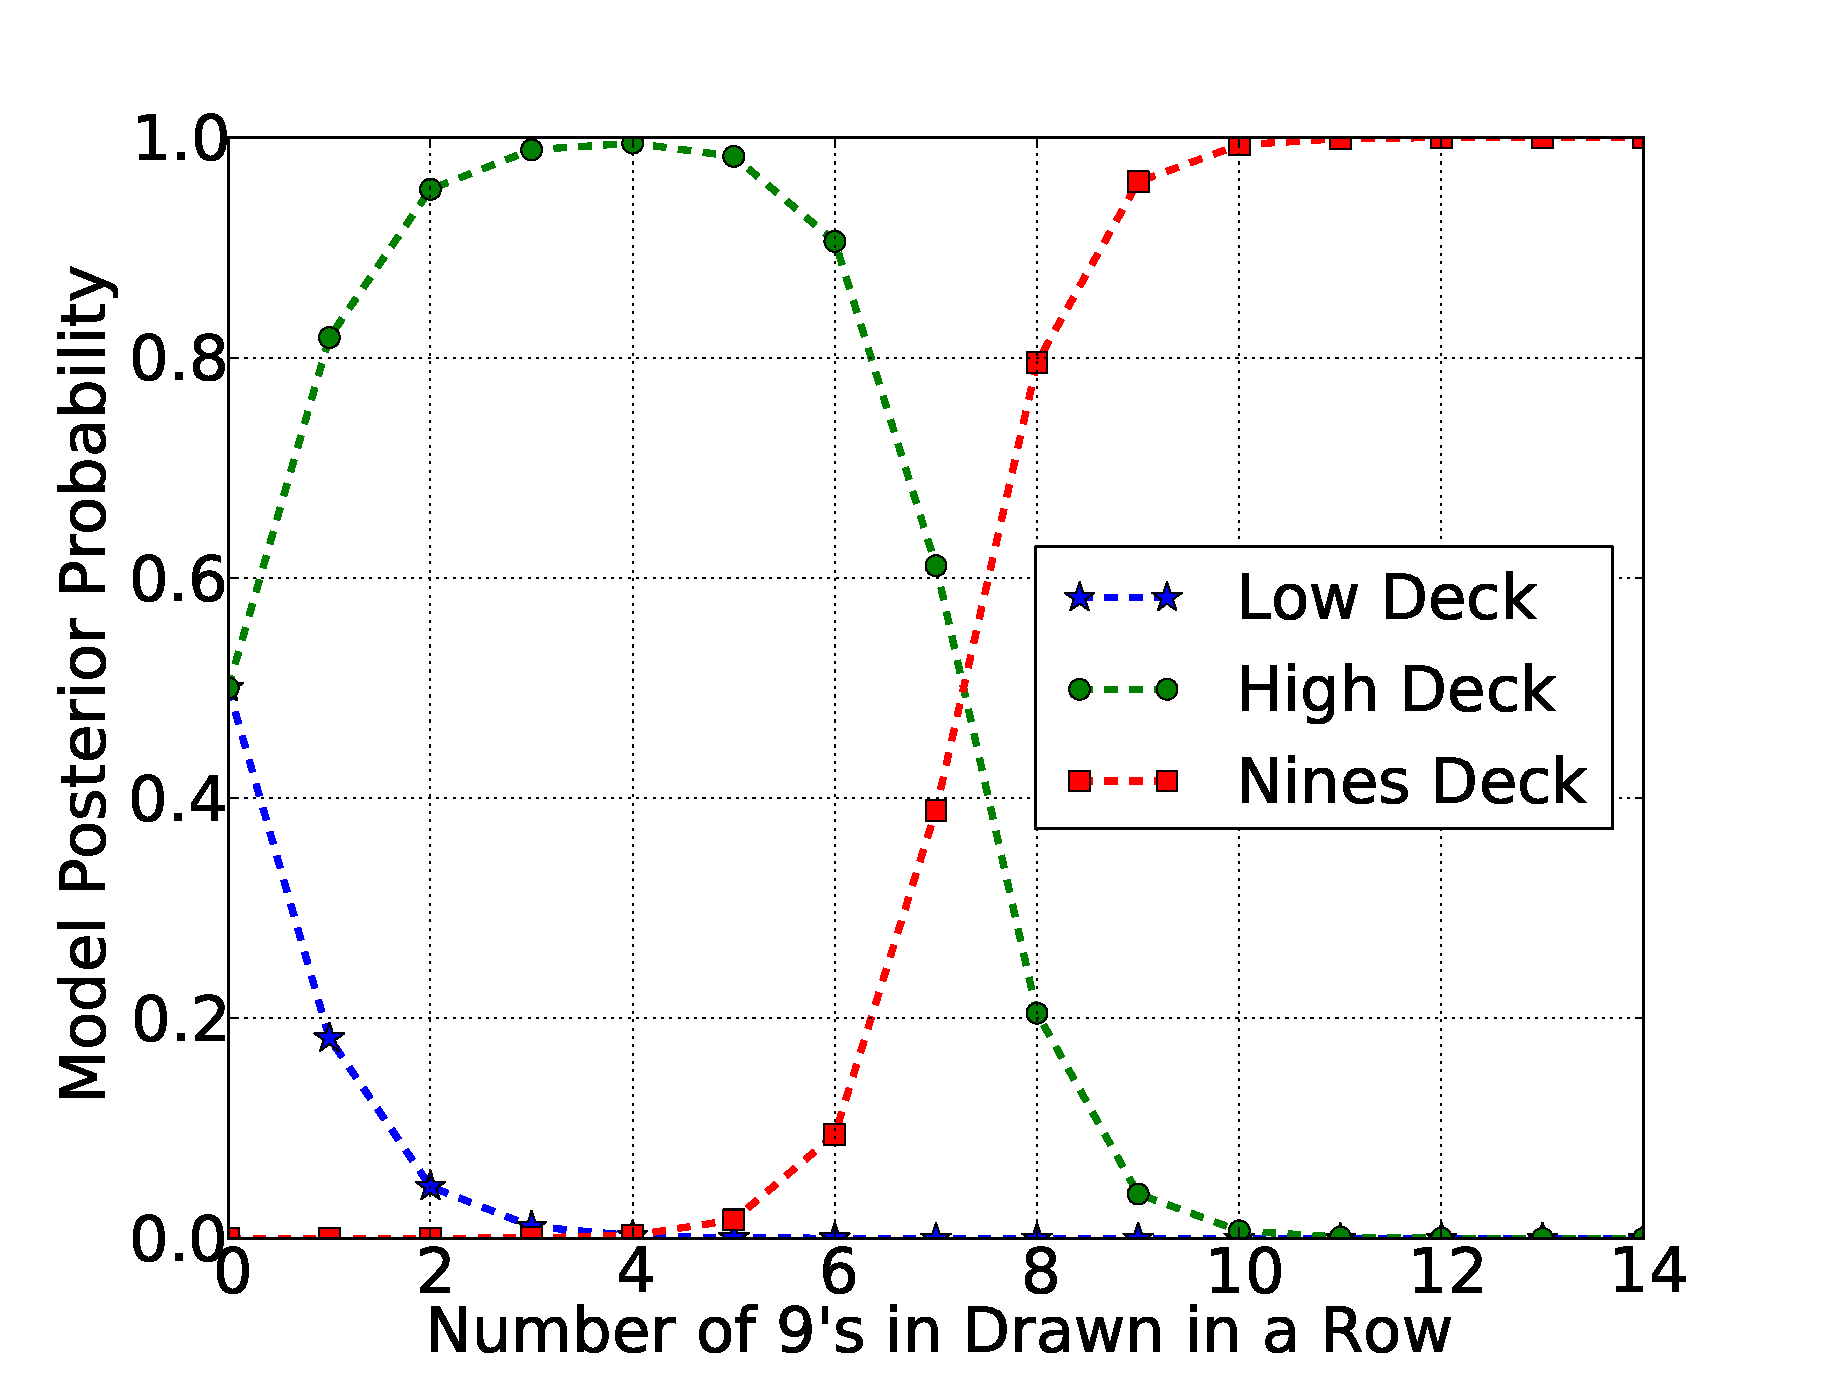
\includegraphics{nines_HLN}
\caption{Drawing a number of 9's in a row, possibly from a High, Low, and Nines deck.}
\label{fig:nines_HLN}
\end{figure}

We have a clear picture here in Figure~\ref{fig:nines_HLN}.  As we initially draw 9's, our confidence that we're holding the High Deck goes up, at the expense of our confidence that we're holding the Low Deck.  At a certain point (around six 9's in our example), our confidence in the High Deck starts to drop and we become more confident that something odd is happening, and our previously ignored model of the Nines deck becomes more likely.  Eventually, this new model is the one in which we are the most confident.  

Imagine further that if, after drawing ten 9's in a row we draw a 1.  What do we do then?  The likelihood for the Nines deck goes to {\em zero} instantly - the probability of drawing a 1 from a Nines deck is zero, $P(1|N)=0$.  Are we left again with the original two models, High and Low Deck?  No!  We would then introduce other models, perhaps something like a Mostly Nines Deck, or perhaps a High Deck with a weird shuffling procedure, or perhaps others\marginnote{The creative part of science is not in the calculations performed, but in the generation of new and useful models.  Until we come up with a better model for our data we make do with the ones that we have, all the while being aware that a better model may come into play later.  Newton's Theory of Gravity was used for over 200 years, even when there was known data that made it less likely, until it was replaced by Einstein's Theory of Gravity.  Newton's Laws, however, are still used in nearly all gravitational calculations because it is ``good enough'' and is a lot easier to work with practically.}.  No matter how many models one has, the recipe is still the same.  It is important to realize that in any model comparison case, there are always other models that could be brought to bear on the problem, perhaps with low prior probability.  Simply showing that a model is consistent with a set of data does not insure against the possibility that another model could be better, if we could only think of it.

\exercise{Drawing a 3}{Complete the example demonstrating the updated probabilities for the High and Low Deck, having drawn a 9, 7, and a 3.  Compare with the case of drawing just the 9 and the 7, and discuss how it matches your intuition.}

\exercise{Nines and an Eight}{
Repeat the analysis of the sequence of 9's drawn in a row with an added hypothesis of a deck with one hundred 9's and one 8.  Discuss the results.  Demonstrate what happens to the probabilities for all of the hypotheses after drawing one 8, after ten 9's in a row.  Discuss.
}

\exercise{Weird Coins}{
I tell you that I have a coin that could have {\em both sides} heads, {\em both sides} tails, or a normal single-heads single-tails coin.  
\be
\i Before seeing the data, what would be a reasonable prior probability for the three hypotheses $H_{0}$ (no-heads), $H_{1}$ (one head), and $H_{2}$ (two heads)?
\i Would this have been different if you had simply been given a coin by a friend to flip to see who has to do the dishes?  Why or why not?
\i Now I flip the coin once, and get a heads.  Write down the {\em likelihood} of this data given each of the models.  In other words, what are the values of:
\bi
\i $\Pg{data=1 heads}{$H_{0}$}$
\i $\Pg{data=1 heads}{$H_{1}$}$
\i $\Pg{data=1 heads}{$H_{2}$}$
\ei
\i Apply Bayes' Recipe, and determine the probability of each of these three models given this data.  In other words, what are the values of:
\bi
\i $\Pg{$H_{0}$}{data=1 heads}$
\i $\Pg{$H_{1}$}{data=1 heads}$
\i $\Pg{$H_{2}$}{data=1 heads}$
\ei
\i Apply this recipe for the case of observing 3 heads in a row.
\ee

}
